\documentclass[11pt]{article}
\usepackage{codenote}

\title{Math5485 - 2026 Fall Group Project}
\author{Yuqiao ZHANG \& Yuran Cheng \& Chengxuan Ku \& Mutian Qi}
\date{\today}

\begin{document}

\maketitle

\section{Problem I: The model problem and Euler’s method}

\subsection{Exercise 1}

\begin{enumerate}
    \item \textbf{(Yuqiao Zhang)} \\ 
    \textbf{Method 1.} Observe that $\dfrac{u'(t)}{u(t)^2} = -\sin t$, then, integrating both side. 
    $$\begin{aligned}
        & \int \dfrac{u'(t)}{u(t)^2} \mathrm{d}t  = - \int \sin t \mathrm{d}t \\ 
        \Longrightarrow &-\dfrac{1}{u(t)} = \cos t + C\\ 
        \Longrightarrow & u(t) = \dfrac{1}{C - \cos t}. 
    \end{aligned}$$
    Therefore, $u(t) = \dfrac{1}{C-\cos t}$, plug the initial value $u(0) = u_0$, then, $$u_0 = \dfrac{1}{C- \cos 0} = \dfrac{1}{C-1} \Longrightarrow C = 1 + \dfrac{1}{u_0}. $$
    Therefore, $$u(t) = \dfrac{1}{1+\dfrac{1}{u_0} - \cos t} = \dfrac{u_0}{u_0 + 1 - u_0 \cos t} = \dfrac{u_0}{(1+u_0) - u_0 \cos t}. $$

    \textbf{Method 2.}  By the quotient rule of $u(t)=\dfrac{u_0}{(1+u_0)-u_0\cos t}$, we obtain that

    $$\begin{aligned}
        u'(t)
        &= -\dfrac{u_0^2\sin t}{\left((1+u_0)-u_0\cos t\right)^2}\\
        &= -\left(\dfrac{u_0}{(1+u_0)-u_0\cos t}\right)^2\sin t\\
        &= -u(t)^2\sin t.
    \end{aligned}$$
    Hence, $u(t)$ satisfies the differential equation. Evaluate at $t = 0$, it can be obtained that $u(0) = \dfrac{u_0}{(1+u_0) - u_0 \cos 0} = u_0$. Thus, we verify that $u(t)$ is a solution of the original differential equation. 

    \item \textbf{(Chengxuan Ku)}  Observe that $0\leq 1-\cos t\leq 2 $, then we consider the following cases. 
    \begin{enumerate}[label=\Roman*. ]
        \item If $u_0\geq 0$, $1+u_0(1-\cos t)\geq 1>0$, then the solution exists for all $t \geq 0$. 
        \item If $u_0 <0$, then $1+u_0(1-\cos t)\geq 1+2u_0$. Thus, if $u_0>-\dfrac12$, the denominator is strictly positive for all $t\geq 0$.
        
        \item If $ u_0=-\dfrac12$, then $u(t) =\dfrac{-\frac12}{1-\frac12(1-\cos t)} =-\dfrac{1}{1+\cos t}.$ At $t=\pi$, the denominator vanishes.
        \item If $u_0<-\dfrac12$, we set $ g(t)=1+u_0(1-\cos t).$then $g(0)=1>0$ and $g(\pi)=1+2u_0<0.$ 
        
        Since $g(t)$ is continuous, by the Intermediate Value Theorem we know there exists a root $T\in(0,\pi)$ and we have $T=\arccos\left(1+\dfrac{1}{u_0}\right)$. Thus, $\displaystyle \lim_{t\to T^-}u(t)=-\infty.$ 
        
        Consequently, the solution blows up in finite time if and only if $u_0\leq-\dfrac{1}{2}$.
    \end{enumerate}
\end{enumerate}

\subsection{Exercise 2} \label{E2}

\begin{enumerate}
    \item \label{E2-1} \textbf{(Mutian Qi)} Consider that u(t) is the solution to differential equation, $u'(t)=f(t,u(t))$. By transforming $t$ to the variable $s$, $u'(s)=f(s,u(s))$. 
    
    Then, by the foundation theorem of calculus, we have $\displaystyle u(t_{j+1})-u(t_j)=\int_{t_j}^{t_{j+1}}u'(s)ds$. By substituting into the differential equation, $$u(t_{j+1})-u(t_j)=\int_{t_j}^{t_{j+1}}u'(s)ds=\int_{t_j}^{t_{j+1}}f(s,u(s))ds, $$ where $u'(s)=f(s,u(s))$, which holds for the statement. 

    
    \item \textbf{(Mutian Qi)} By part(a), we already proved that $\displaystyle u(t_{j+1})-u(t_j)=\int_{t_j}^{t_{j+1}}f(s,u(s))ds$. Let $h$ be the width satisfying that $h=t_{j+1}-t_j$, we have 
    $$\displaystyle \int_{t_j}^{t_{j+1}}f(s,u(s))ds\approx hf(t_j,u(t_j))$$ 
    in which the height is $f(t_j,u(t_j))$. So, $u(t_{j+1})-u(t_j)\approx hf(t_j,u(t_j))$, which $u_j\approx u(t_j),u_{j+1}\approx u(t_{j+1})$. So, $u_{j+1}-u_j\approx hf(t_j,u_j)$, which gives us that $u_{j+1}=u_j+hf(t_j,u_j)$, for which $j=0,...,n-1$ in which $u_0=u(0)$, which holds for the Euler's Method.


    \item \textbf{(Yuran Cheng)} For $u_0=1$ and $T=2$, the exact solution is
    \[
        u(t)=\frac{1}{2-\cos t}.
    \]
    Euler's method with $h=2/n$ gives
    \[
        u_{j+1}=u_j+h f(t_j,u_j)
        =u_j-hu_j^2\sin t_j,
        \qquad t_j=jh,\quad u_0=1.
    \]
    We apply the method with $n=5,10,100$ and compare the numerical
    solutions with the exact solution in the figure below.

    \inputcode{code/exercise2-3.py}

    
    \begin{center}
        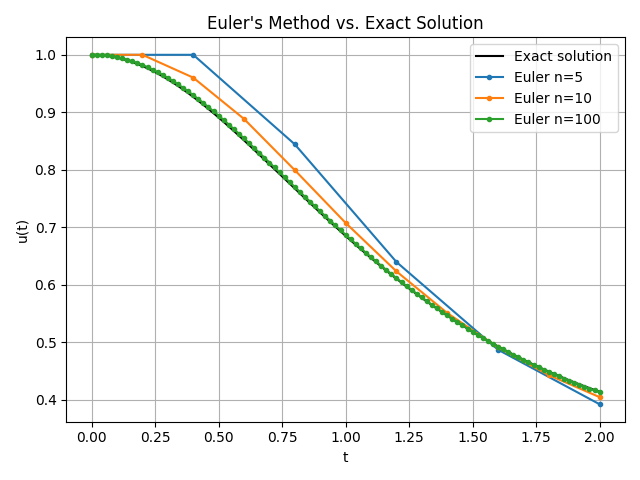
\includegraphics[width=0.8\textwidth]{picture/exercise2-3.png}
    \end{center}
    As $n$ increases, the numerical approximations become closer to the
    exact solution. In particular, the approximation for $n=100$ is
    much more accurate than those for $n=5$ and $n=10$.

    \item \textbf{(Yuran Cheng)}
    For each $n=1,\ldots,500$, we compute the maximum error
    \[
        e_n=\max_{0\le j\le n}|u_j-u(t_j)|,
        \qquad t_j=\frac{2j}{n}.
    \]
    The errors are plotted against $n$ on a log--log scale.
    \begin{center}
        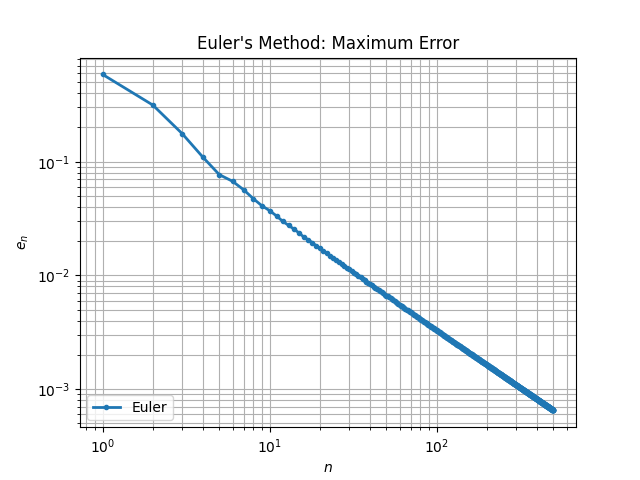
\includegraphics[width=0.8\textwidth]{picture/exercise2-4.png}
    \end{center}
    The error decreases approximately as $n^{-1}$. Since $h=2/n$,
    this is consistent with the first-order convergence of Euler's method:
    \[
        \boxed{e_n=O(n^{-1})=O(h),\qquad r=1.}
    \]
    \item \textbf{(Chengxuan Ku)} We can set $u_j=u(t_j)$ exactly, 
    $$
     u(t_{j+1})=u(t_j)+\int_{t_j}^{t_{j+1}}f(s,u(s))\mathrm{d}s,
     \qquad u_{j+1}=u(t_j)+hf(t_j,u(t_j)).
    $$
    Let $g(s)=f(s,u(s))=u'(s)$. Then by rectangular rule estimate we have
    $$
     |u_{j+1}-u(t_{j+1})|=\left|hg(t_j)-\int_{t_j}^{t_{j+1}}g(s)\mathrm{d}s \right|\le\frac{h^2}{2}\max_{s\in[t_j,t_{j+1}]}|g'(s)|.
    $$
    By the chain rule,
    $g'(s)=f_t(s,u(s))+f_u(s,u(s))u'(s)=u''(s).$ 
    
    Therefore,
    $$|u_{j+1}-u(t_{j+1})|\le\frac{h^2}{2}\max_{s\in[t_j,t_{j+1}]}|u''(s)|. $$

We know there are $n=\dfrac{T}{h}$ steps. If the propagation of errors is stable, summing $n$ local contributions of order $h^2$ with bounded error amplification leads to a global error of order $nO(h^2)=O(h)=O(n^{-1})$. This is consistent with (iv).

    \item \textbf{(Yuran Cheng)}
    Consider the initial value problem
    \[
        u'(t)=\mu u(t),\qquad u(0)=1.
    \]
    The function $u(t)=e^{\mu t}$ satisfies
    \[
        u'(t)=\mu e^{\mu t}=\mu u(t),\qquad u(0)=1,
    \]
    so it is the exact solution.
    
    For Euler's method, let $h=T/n$. Then
    \[
        u_{j+1}=u_j+h\mu u_j=(1+\mu h)u_j.
    \]
    Since $u_0=1$, repeated application yields
    \[
        \boxed{u_n=(1+\mu h)^n
        =\left(1+\frac{\mu T}{n}\right)^n.}
    \]
    To determine the rate of convergence, set $a=\mu T$. Using
    $\log(1+x)=x-x^2/2+O(x^3)$ as $x\to0$, we obtain
    \[
        n\log\left(1+\frac{a}{n}\right)
        =a-\frac{a^2}{2n}+O(n^{-2}).
    \]
    Consequently,
    \[
        \left(1+\frac{a}{n}\right)^n
        =e^a\left(1-\frac{a^2}{2n}+O(n^{-2})\right).
    \]
    It follows that
    \[
        \boxed{\left|e^{\mu T}-u_n\right|
          =\frac{e^{\mu T}(\mu T)^2}{2n}+O(n^{-2}).}
    \]
    Therefore, if $\mu T\ne0$, the error is asymptotically
    proportional to $n^{-1}$, so Euler's method converges with
    \textbf{order $r=1$}. If $\mu T=0$, the approximation is exact
    for every $n$.
    \begin{center}
        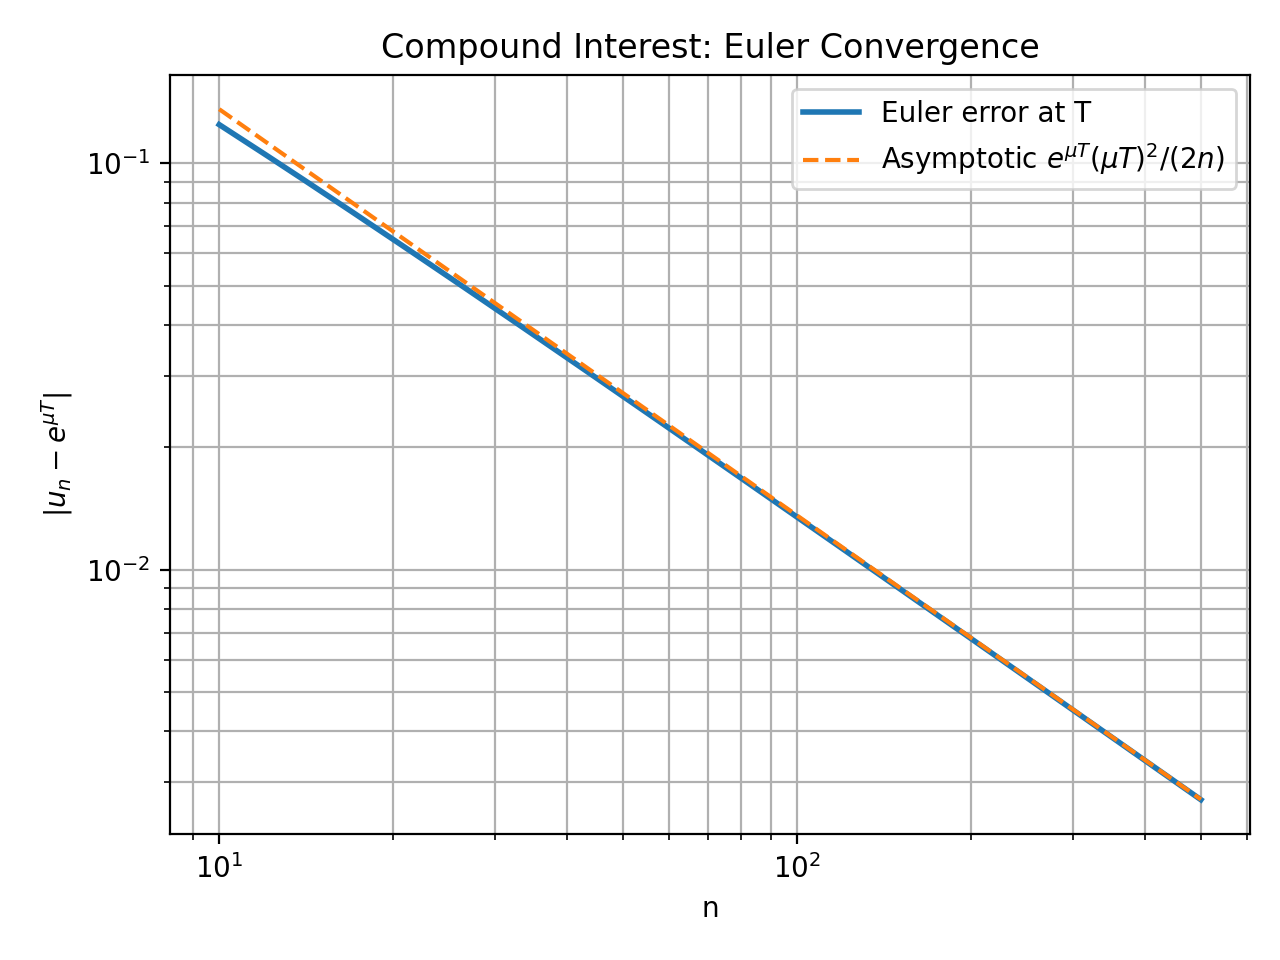
\includegraphics[width=0.8\textwidth]{picture/exercise2-6.png}
    \end{center}
\end{enumerate}

\section{Problem II: Implicit and other methods}

\subsection{Exercise 3} 

\begin{enumerate}
    \item \label{E3-1} \textbf{(Yuqiao Zhang)} Accoding to \ref{E2}.\ref{E2-1}, we have $\displaystyle u(t_{j+1})=u(t_j)+\int_{t_j}^{t_{j+1}}f(s,u(s)) \mathrm{d}s$.

            Recall the Trapeziod Rule that for a function $g(s)$, we have $\displaystyle \int_a^b g(s) \mathrm{d}s \approx \dfrac{b-a}{2} \left[g(a) + g(b)\right]$. Let $g(s) = f\left(s ,u(s)\right)$, then $$u\left(t_{j+1}\right) - u \left(t_j \right) \approx  \dfrac{h}{2} \left[f\left(t_j,u\left(t_j\right)\right) + f\left(t_{j+1},u\left(t_{j+1}\right)\right)\right]. $$

            Use $u_j \approx u\left(t_j\right)$ and $u_{j+1} \approx t\left(t_{j+1}\right)$, we derive that $u_{j+1}=u_j+\dfrac{h}{2} \left[f\left(t_j,u_j\right)+f\left(t_{j+1},u_{j+1}\right)\right]$. 

            By using the \href{https://jackrthomas.github.io/Math5485/lectures/L10.html\#trapezoid-rule}{Theorem 10.3}, if $g \in C^2 \left(\left[0, T\right]\right)$, the error estimate of composite trapeziod rule satisfied with $$\left| E_n \right| \le \dfrac{\|g''\|_\infty}{12}\dfrac{T^3}{n^2} = \dfrac{T\|g''\|_\infty}{12}h^2, $$ where $h = \dfrac{T}{n}$. Therefore, we expect the convergence rate is $O\left(h^2\right) = O\left(n^{-2}\right)$. 

    \item \textbf{(Yuqiao Zhang)} \\ 
        \textbf{Method 1.} Substituting $f(t,u)=-u^2\sin t$ into (7), we obtain
        $$u_{j+1}=u_j-\dfrac{h}{2} \left[u_j^2\sin(t_j)+u_{j+1}^2\sin(t_{j+1})\right].$$

        Then, $u_{j+1}+\dfrac{h}{2}\sin(t_{j+1})u_{j+1}^2 +\left(\dfrac{h}{2}\sin(t_j)u_j-1\right)u_j=0.$

        By the definition of $\Phi$, we have $\Phi(u_{j+1})=0$. 

        \textbf{Method 2.} Define the residual of (7) by $R(v)=v-u_j-\dfrac{h}{2} [f(t_j,u_j)+f(t_{j+1},v)]$. Since $f(t,u) = -u^2 \sin t$, we have $R'(v)=1+hv\sin(t_{j+1})=\Phi'(v)$. 

        Then, we have $R(0)=-u_j+\dfrac h2u_j^2\sin(t_j)=\Phi(0)$.  Since $R'=\Phi'$ and $R(0)=\Phi(0)$, we obtain that $R(v)=\Phi(v)$ for all $v$. Thereby, $R(u_{j+1})=0$ if and only if $\Phi(u_{j+1})=0$. 
    
    \item \textbf{(Yuqiao Zhang)} \\ 
        \textbf{Method 1.} From (8), we have $\Phi'(v)=1+h\sin(t_{j+1})v$ and $\Phi''(v)=h\sin(t_{j+1})$. 

        Consider $I=[u_j-1,u_j+1]$, assuming $|u_j|$ remains bounded as $h\to0$. For sufficiently small $h$, we have $\Phi(u_j\pm1)=\pm 1+O(h)$. Also , $\Phi'(v)\ge1-h(|u_j|+1)\ge\dfrac12>0$, $v \in I$.  Hence, $\Phi$ has a unique simple root $r\in I$.

        Then, $\Phi(u_j)=O(h)$, $v_1-u_j=O(h)$. 
        
        By using the Mean Value Theorem, $|r-u_j|\le2|\Phi(u_j)|=O(h).$ Thus, $|v_1-r|=O(h)$. 

        For all $x, y \in I$, $\left|\dfrac{\Phi''(x)}{\Phi'(y)}\right| \le2h\longrightarrow0$ as $h\to0.$ Taking $A=2h$, we have, for sufficiently small $h$, $|v_1-r|\le A^{-1}=\dfrac1{2h}$. Therefore, by \href{https://jackrthomas.github.io/Math5485/lectures/L05.html#newton}{Theorem 5.3}, Newton's method converges at least quadratically to $r=u_{j+1}$, where $\Phi(u_{j+1})=0$.

        \textbf{Method 2.} The Newton's iteration is $v_{k+1}=v_k-\dfrac{\Phi(v_k)}{\Phi'(v_k)}.$

        Since $\Phi$ is quadratic, Taylor's expansion is exact for 
        $$
        \Phi(v_{k+1})
        =\Phi(v_k)+\Phi'(v_k)(v_{k+1}-v_k) +\dfrac{h\sin(t_{j+1})}{2}(v_{k+1}-v_k)^2
        =\dfrac{h\sin(t_{j+1})}{2} \left(\dfrac{\Phi(v_k)}{\Phi'(v_k)}\right)^2.
        $$
        For sufficiently small $h$, on
        $I=[v_1-1,v_1+1]$, we have $\dfrac{1}{2} \le \Phi'(v) \le \dfrac{3}{2}.$ Consequently, whenever $v_k\in I$, $|\Phi(v_{k+1})|\le2h|\Phi(v_k)|^2$, $|v_{k+1}-v_k|\le2|\Phi(v_k)|$. 
        
        Using $v_1=u_j-hu_j^2\sin(t_j)$, $\Phi(v_1)=\dfrac{h}{2} \left[\sin(t_{j+1})v_1^2-\sin(t_j)u_j^2\right].$
        
        Since $|\sin(t_{j+1})-\sin(t_j)|\le h$ and $|v_1-u_j|\le hu_j^2$, 
        $$|\Phi(v_1)| \le\dfrac h2\left[hu_j^2+|v_1-u_j||v_1+u_j|\right] \le\dfrac{h^2}{2}\left[u_j^2+2|u_j|^3+hu_j^4\right]=O(h^2).$$
        
        Choose $h$ sufficiently small so that $2h|\Phi(v_1)|\le\dfrac12$ and $4|\Phi(v_1)|<1.$
        
        Then, by induction, $|\Phi(v_k)|\le2^{-(k-1)}|\Phi(v_1)|$ and $\displaystyle |v_k-v_1|\le2\sum_{m=1}^{k-1}|\Phi(v_m)|<4|\Phi(v_1)|<1.$
        
        Thus all iterates remain in $I$, and
        $\displaystyle \sum_{k=1}^{\infty}|v_{k+1}-v_k|\le 4|\Phi(v_1)|$. Then, the sequence $\left\{v_k\right\}$ is Cauchy and converges to some $u_{j+1}\in I$. By continuity,
        $\displaystyle \Phi(u_{j+1}) =\lim_{k\to\infty}\Phi(v_k)=0.$
        
        By the Mean Value Theorem,
        $\dfrac12|v_k-u_{j+1}| \le|\Phi(v_k)| \le\dfrac32|v_k-u_{j+1}|. $
        
        Therefore,
        $$
        \begin{aligned}
        |v_{k+1}-u_{j+1}|
        &\le2|\Phi(v_{k+1})|\\
        &\le4h|\Phi(v_k)|^2\\
        &\le9h|v_k-u_{j+1}|^2.
        \end{aligned}
        $$
        
        Thus, Newton's method converges at least
        quadratically to $u_{j+1}$.
        
    \item \textbf{(Chengxuan Ku)}The general equation and its derivative for use inside Newton's method are
$$
 F(v)=v-u_j-\frac h2[f(t_j,u_j)+f(t_{j+1},v)] \text{ and }
 F'(v)=1-\frac h2 f_u(t_{j+1},v).
$$  We use them to plot our approximation, the plot is following.
 \begin{center}
        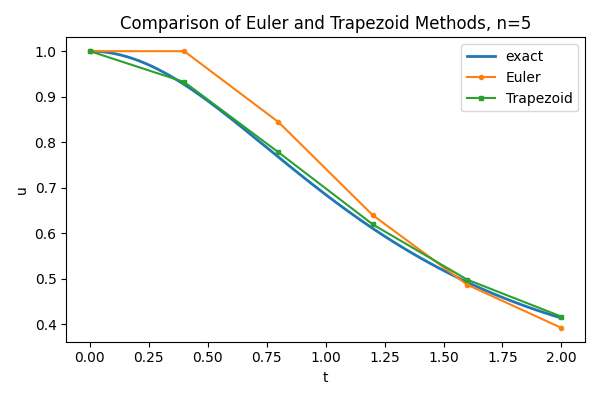
\includegraphics[width=0.8\textwidth]{picture/Exercise 3-4.png}
    \end{center}
 The plot compares the exact solution with the Euler and trapezoidal approximations for $u_0=1, T=2, n=5$. Both numerical methods follow the overall decreasing trend of the exact solution, but the trapezoidal approximation stays closer to the exact curve. It is consistent with its expected second-order convergence compared with the first-order Euler method.  
    \item \textbf{(Yuran Cheng)} For $u_0=1$ and $T=2$, the exact solution is
    \[
        u(t)=\frac{1}{2-\cos t}.
    \]
    With $h=2/n$, the implicit trapezoid method is
    \[
        u_{j+1}=u_j+\frac{h}{2}\bigl[f(t_j,u_j)+f(t_{j+1},u_{j+1})\bigr].
    \]
    At each time step, we solve the implicit equation using Newton's method.
    For $n=1,\ldots,500$, we compute
    \[
        e_n=\max_{0\le j\le n}|u_j-u(t_j)|
    \]
    for both Euler's method and the trapezoid method.
    \begin{center}
        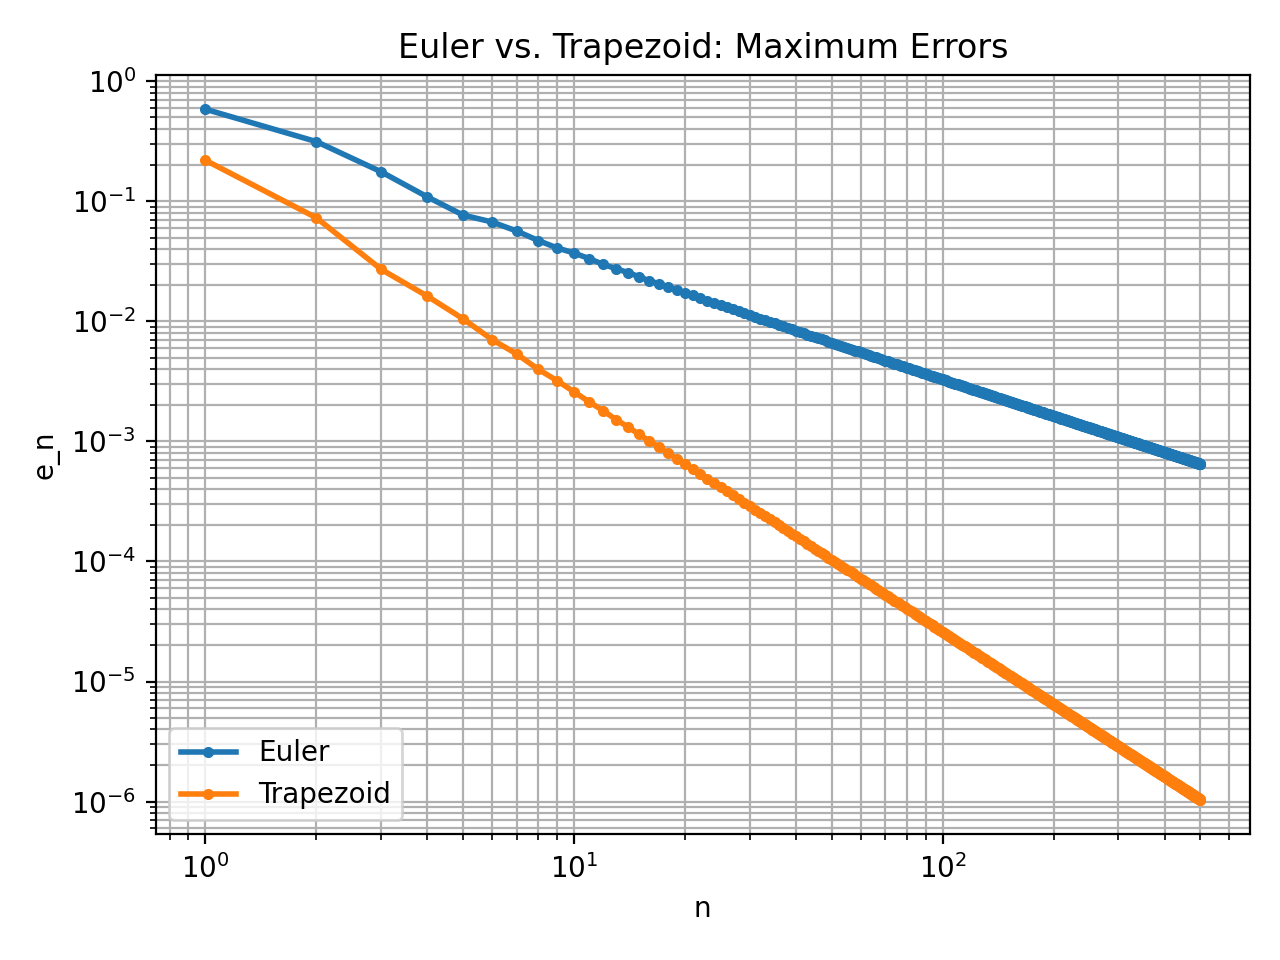
\includegraphics[width=0.8\textwidth]{picture/exercise3-5.png}
    \end{center}
    The log--log plot shows that the trapezoid error decreases approximately
    as $n^{-2}$, whereas Euler's error decreases approximately as $n^{-1}$.
    Thus, the trapezoid method has convergence rate
    \[
        \boxed{r=2,\qquad e_n=O(n^{-2})=O(h^2).}
    \]
    This agrees with part (i), where the trapezoid method was predicted
    to be second-order accurate.
\end{enumerate}


\subsection{Exercise 4}

\begin{enumerate}
    \item \textbf{(Yuqiao Zhang)}  \\ 
    By the definition of $G$ and $f(t,u)=-u^2\sin t$, we have $$G(v)=u_j-\dfrac h2\left[u_j^2\sin(t_j)+v^2\sin(t_{j+1})\right].$$

    After Differentiating, we obtain $G'(v)=-hv\sin(t_{j+1}).$

    Consider $I=[u_j-1,u_j+1]$. Since $|u_j|\le2$, for all $v\in I$, we have $|v|\le |u_j|+1\le3$. Therefore, $|G'(v)|=h|v||\sin(t_{j+1})|\le3h.$

    For any $x,y\in I$, by the Mean Value Theorem, $|G(x)-G(y)|\le3h|x-y|.$

    Thus, whenever $0<h<\dfrac13$, $G$ satisfies the contraction. For all $v\in I$,
    $$\begin{aligned}
        |G(v)-u_j|
        &\le\dfrac h2\left[|u_j|^2+|v|^2\right]\\
        &\le\dfrac h2(4+9)
        =\dfrac{13h}{2}.
    \end{aligned}$$

    Hence, if $0 < h \le \dfrac{2}{13}$, then $G(v) \in I$ for every $v\in I$. Therefore, for all sufficiently small $h$, $G:I\to I$ is a contraction. According to the Banach Fixed-Point Theorem, $G$ has a unique fixed point in $I$, and the iteration $v_{k+1}=G(v_k)$ converges to this fixed point for any $v_1\in I$.
    
    \item \textbf{(Yuran Cheng)}
\end{enumerate}

\section{Problem III: Runge–Kutta and comparing the methods}

\subsection{Exercise 5}

\begin{enumerate}
    \item \textbf{(Yuqiao Zhang)} 
    \item \textbf{(Mutian Qi \& Chengxuan Ku )}
    \begin{enumerate}[label=\Roman*. ]
        \item \textbf{(Chengxuan Ku--Coding)}
        Euler's method need one evaluation of f per step, Heun's method need 2 evaluations, and RK4 need 4 evaluations. We check these counts using the counted function. To compare their efficiency, we plot the maximum error $e_n$ against the total number of evaluations on a log-log scale. The plot is following.
         \begin{center}
        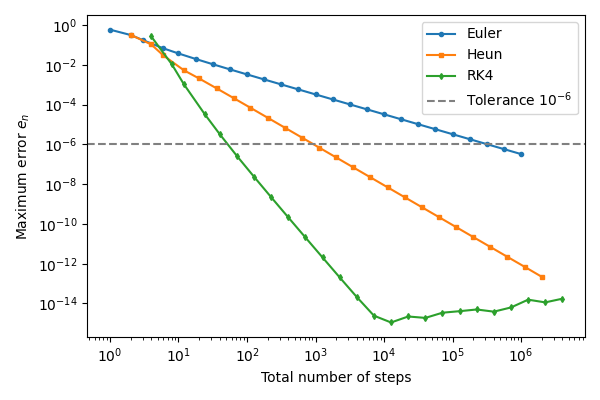
\includegraphics[width=0.8\textwidth]{picture/Exercise 5-2.png}
    \end{center}
        %  不要用中文的逗号，刚才报错是因为这个
        \item \textbf{(Mutian Qi--Writing)} For calculating Euler, we take about $n$ times, while we take $2n$ and $4n$ times separately on Heun and RK4. Based on the plot of error, the function takes 8 steps of calculation, and it takes 4 times in each of 8 steps, so total evaluations should be 32 times. In this case, we prefer RK4 because RK4 is 4th order method. Even if each steps take calculation over quartic function, the error declines faster. 

        
        
    \end{enumerate}
\end{enumerate}

\section{Problem IV: OPTIONAL SECTIONS}

\subsection{Optional 1. \textbf{(Yuqiao Zhang)}}



\end{document}


